% $Id: DesignPatterns.tex,v 1.1 2008/01/31 18:04:16 dconway Exp $
\chapter{\label{chapter:Patterns}Design Patterms Used in GMAT}
\chapauthor{Darrel J. Conway}{Thinking Systems, Inc.}

The GMAT design was influenced by many different sources: prior experience with Swingby, Navigator,
FreeFlyer, and Astrogator, exposure to analysis and operational systems for Indostar, Clementine,
WIND, ACE, and SOHO, and design experiences on other software projects.  Part of the theoretical
background for the GMAT design comes from exposure to the object oriented design community,
captured in the writings of Scott Meyers, Herb Sutter, Bruce Eckel, Martin Fowler, and the Gang of
Four\cite{GoF}.

This latter reference provides a framework for describing recurrent patterns in software systems.
Patterns that are used by reference in this document are summarized here for completeness; avid
readers will also want to read the Gang of Four text or a similar book derived from it.

\section{\label{section:TheSingletonPattern}The Singleton Pattern}

\subsection{Motivation}
Some of the components of GMAT require implementation such that one and only one instance of the
component exist.  Examples of these components are the Moderator, the ScriptInterpreter, the
Publisher, the ConfigurationManager, and the FactoryManager.  These objects are implemented using
the Singleton design pattern.

\begin{figure}[htb]
\begin{center}
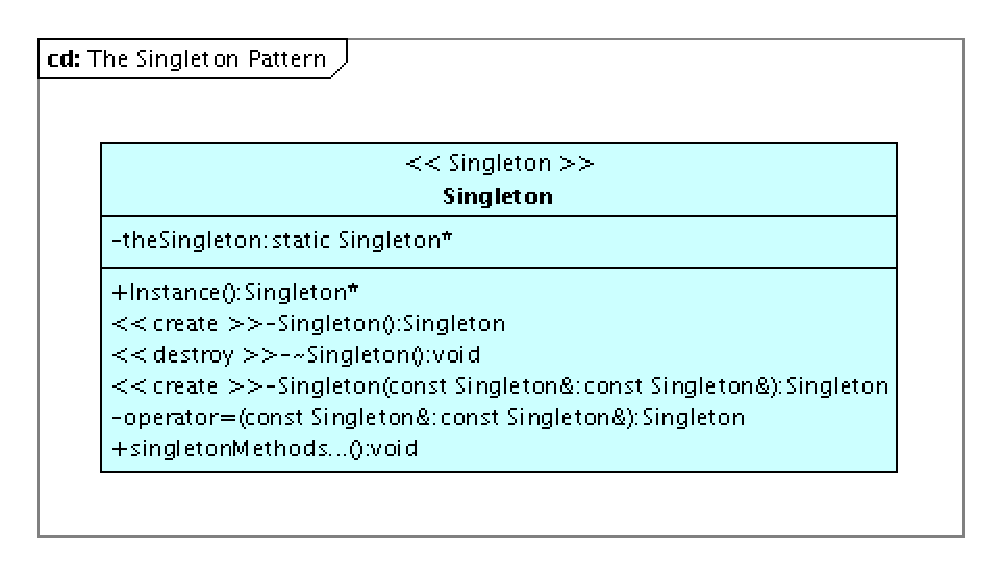
\includegraphics[scale=0.5]{Images/TheSingletonPattern.eps}
\caption{\label{figure:TheSingletonPattern}Structure of a Singleton}
\end{center}
\end{figure}

\subsection{Implementation}

Figure~\ref{figure:TheSingletonPattern} shows the key elements of a singleton.  The class is
defined so that there is only one possible instance during the program's execution.  This instance
is embodied in a private static pointer to a class instance; in the figure, this pointer is the
``theSingleton'' member.  This pointer is initialized to NULL, and set the first time the singleton
is accessed.

The class constructor, copy constructor, assignment operator, and destructor are all private in
scope.  The copy constructor and assignment operator are often declared but not implemented, since
they cannot be used in practice for singleton objects.  All access to the Singleton is made through
the Instance() method.

The first time Instance() is called, the pointer to the singleton is constructed.  Subsequent calls
to Instance() simply return the static pointer that was set on the first call.  A sample
implementation of the Instance() method is shown here:

\begin{quote}
\begin{verbatim}
Singleton* Instance()
{
   if (theSingleton == NULL)
      theSingleton = new Singleton();
   return theSingleton;
}
\end{verbatim}
\end{quote}

\subsection{Notes}

In GMAT, the Singletons are all terminal nodes in the class hierarchy.  Some designs allow
subclassing of Singletons so that the final singleton type can be selected at run time.  GMAT does
not subclass its singletons at this time.

\section{The Factory Pattern}

\subsection{Motivation}

The Factory design pattern -- sometimes called the Factory Method, defines an interface for creating
objects, and uses that interface in subclasses to create objects os specific types.  GMAT uses this
pattern for user created objects.  The Factory base class specifies the creation interfaces into
GMAT's factories.  Derived factory classes override the interfaces specific to the type of factory
that is being implemented.

\subsection{Implementation}

The factory classes as implemented in GMAT are discussed, with sample code, in
Section~\ref{section:FactoryClasses}.  Please refer to that section for implementation details.

\section{The Observer Pattern}


\section{\label{section:MediatorPattern}The Mediator Pattern}

\subsection{Motivation}

The Mediator design pattern centralizes the communications between objects into a single component.
 This consolidation of the communications simplifies the interfaces that the mediator's clients
need to support, and helps decouple the objects from one another.  Additionally, the interfaces can
be made more consistent by keeping the Mediator interfaces consistent.

\subsection{Implementation}

GMAT uses the Mediator pattern in the engine code.  The Moderator is the mediator for GMAT's
engine.  Details of the implementation for the Moderator are in Chapter~\ref{chapter:Moderator}.

\subsection{Notes}

The colmmon terminology in the literature refers to the mediator as the core class for the Mediator
pattern, and calls the classes that are mediated ``Colleagues.''  For the GMAT engine, the Mediator
is the Moderator, and the Colleagues are the Factory Manager, the Configuration Manager, and the
Sandboxes.

\section{\label{section:TheAdapterPattern}The Adapter Pattern}

GMAT uses adapters to simplify invocation of calculations on different types of objects, making the
interface identical even though the underlying classes are quite different.  One example of the use
of adapters in GMAT is the ElementWrapper classes used by the command subsystem.  Many of the
commands in GMAT need a source of Real data in order to function correctly.  This data can be
supplied as a number, an object property, a GMAT Parameter, an Array element, or any other source of
Real data in the system.  ElementWrappers encapsulate the disparate interfaces to these objects so
that the commands can use a single call to obtain the Real data, regardless of the underlying
object.

\section{\label{section:TheMVCPattern}The Model-View-Controller (MVC) Pattern}
